% !TEX options=--shell-escape
% https://github.com/SublimeText/LaTeXTools/issues/1082
%  _____ _             _    ______             __ _ __  
% |  ___(_)_ __   __ _| |  / /  _ \ _ __ __ _ / _| |\ \ 
% | |_  | | '_ \ / _` | | | || | | | '__/ _` | |_| __| |
% |  _| | | | | | (_| | | | || |_| | | | (_| |  _| |_| |
% |_|   |_|_| |_|\__,_|_| | ||____/|_|  \__,_|_|  \__| |
%                          \_\                      /_/ 
                   
% -------------------------------------------------------------------------
% https://www.kammerl.de/ascii/AsciiSignature.php - standard
% I've moved beyond justifying latex and am not just living in it.


% Use APA module
% Based on template from https://www.overleaf.com/latex/templates/your-apa6-style-manuscript/kngbbqpypjcq
\documentclass[a4paper,man,natbib]{apa6}
% Imports natbib
% Ref Sheet: https://gking.harvard.edu/files/natnotes2.pdf

% Packages
\usepackage[english]{babel}
\usepackage[utf8x]{inputenc}
\usepackage{amsmath}
\usepackage{graphicx}
% set single spacing
\usepackage{setspace}
% glossary
\usepackage[acronym]{glossaries}
% fancy quotes
\usepackage{epigraph, varwidth}
% For formatting of potential bibliography
\usepackage{enumitem}
% html links
\usepackage{hyperref}
%\usepackage[colorinlistoftodos]{todonotes}
% Allow seperate footnotes
\usepackage{sepfootnotes}
% Diagrams!
\usepackage{svg}
\usepackage{graphicx}
\graphicspath{ {images/} }

% Trying to include graphics has been a JOURNEY
% Links used:
% aborted attempt to use svgs
% https://tex.stackexchange.com/questions/542766/inkscape-1-0-not-able-to-export-files-needed-for-svg-package
% https://tex.stackexchange.com/questions/2099/how-to-include-svg-diagrams-in-latex
% (updated comand line is: inkscape -D --export-latex  "EDEN_diagram.svg" --export-type="pdf" --export-filename="EDEN_diagram_svg-tex.pdf")
% https://www.overleaf.com/learn/latex/Inserting_Images
% convert EDEN_diagram.png -resize 50% EDEN_diagram.png


% This section was found in a stack overflow comment about making the epigraph length different and I include it here as an incantation against bad formatting
\renewcommand{\epigraphsize}{\small}
\setlength{\epigraphwidth}{0.6\textwidth}
\renewcommand{\textflush}{flushright}
\renewcommand{\sourceflush}{flushright}
% A useful addition
\newcommand{\epitextfont}{\itshape}
\newcommand{\episourcefont}{\scshape}

\makeatletter
\newsavebox{\epi@textbox}
\newsavebox{\epi@sourcebox}
\newlength\epi@finalwidth
\renewcommand{\epigraph}[2]{%
  \vspace{\beforeepigraphskip}
  {\epigraphsize\begin{\epigraphflush}
   \epi@finalwidth=\z@
   \sbox\epi@textbox{%
     \varwidth{\epigraphwidth}
     \begin{\textflush}\epitextfont#1\end{\textflush}
     \endvarwidth
   }%
   \epi@finalwidth=\wd\epi@textbox
   \sbox\epi@sourcebox{%
     \varwidth{\epigraphwidth}
     \begin{\sourceflush}\episourcefont#2\end{\sourceflush}%
     \endvarwidth
   }%
   \ifdim\wd\epi@sourcebox>\epi@finalwidth 
     \epi@finalwidth=\wd\epi@sourcebox
   \fi
   \leavevmode\vbox{
     \hb@xt@\epi@finalwidth{\hfil\box\epi@textbox}
     \vskip1.75ex
     \hrule height \epigraphrule
     \vskip.75ex
     \hb@xt@\epi@finalwidth{\hfil\box\epi@sourcebox}
   }%
   \end{\epigraphflush}
   \vspace{\afterepigraphskip}}}
\makeatother
% End epigraph modifications

\makenoidxglossaries
% These used to be in a seperate file, but I want them in here because it will let me cite things from the bibliography in them

%   _____ _                                
%  / ____| |                               
% | |  __| | ___  ___ ___  __ _ _ __ _   _ 
% | | |_ | |/ _ \/ __/ __|/ _` | '__| | | |
% | |__| | | (_) \__ \__ \ (_| | |  | |_| |
%  \_____|_|\___/|___/___/\__,_|_|   \__, |
%                                     __/ |
%                                    |___/ 


\newacronym{foss}{FOSS}{Free Open Source Software}
\newacronym{sts}{STS}{Science, Technology \& Society}
\newacronym{ict}{ICT}{Information and Communications Technology}
\newacronym{eden}{EDEN}{Emergency Development ENvironment}
\newacronym{ict4d}{ICT4D}{Information and Communication Technologies for Development}


\newglossaryentry{ICT}
{
    name=Information and communications technology,
    description={Information and communications technology: A term for the mix of physical devices and software that mix analog and digital techniques to allow communication, recall and storage of data.}
}
 
\newglossaryentry{FOSS}
{
    name=Free Open Source Software,
    description={Free Open Source Software: A method of developing software that does not charge for use of the software. The software's source code is also freely distributed, allowing users to modify their copy of the software or suggest changes to the organization developing it.}
}

\newglossaryentry{python}
{
    name=python,
    description={Python is an open source, interpreted, high-level, general-purpose programming language. It was initially released in the early 1990s, but has been continuously updated since then. Python 2 was the standard from 2000 to 2008, but in 2008 Python 3 was released with backwards-incompatible changes. This split the Python community, leading to Python 2 and Python 3 having slightly different versions of tools available. Python 2 continued to receive support and updates until 2020, when official support for Python ended (Wikipedia contributors, 2020). The open source nature of Python means that it is likely that Python 2 will continue to be updated by users after official support ends. }
}

\newglossaryentry{OpenStreetMap}
{
    name=OpenStreetMap,
    description={An open community of volunteers that maintain data about roads, trails, cafés, railway stations, and much more, all over the world.}
}
\newglossaryentry{web framework}
{
    name=web framework,
    description={A heterogeneous set of software that allow a programmer to efficiently write and manage providing a service over the Internet. This could be a website or a mobile app (often it is both) or a go-between for other services. Examples include web2py and Django in Python or Phoenix in Elixir.}
}

\newglossaryentry{PostgreSQL}
{
   name=PostgreSQL,
   description={PostgreSQL is a powerful, open source object-relational database system with over 30 years of active development that has earned it a strong reputation for reliability, feature robustness, and performance.}
   % https://www.postgresql.org/
}

% https://en.wikipedia.org/wiki/MySQL
%  MySQL is a component of the LAMP web application software stack (and others), which is an acronym for Linux, Apache, MySQL, Perl/PHP/Python. MySQL is used by many database-driven web applications, including Drupal, Joomla, phpBB, and WordPress
\newglossaryentry{MySQL}
{
   name=MySQL,
   description={MySQL is an open-source relational database management system (RDBMS). Its name is a combination of "My", the name of co-founder Michael Widenius's daughter, and "SQL", the abbreviation for Structured Query Language}
}

% http://eden.sahanafoundation.org/wiki/WikiStart#WhatisSahanaEden
\newglossaryentry{EDEN}
{
   name=EDEN,
   description={The Emergency Development ENvironment, developed by the Sahana Foundation, is an Open Source Humanitarian Platform which can be used to provide solutions for Disaster Management, Development, and Environmental Management sectors}
}

\newglossaryentry{ICT4D}
{
   name=Information and Communication Technologies for Development,
   description={The movement to use digital technologies to serve the needs of the underprivileged and those living in the developing world. Criticized for being directed more at the developed worlds' love of technology than the actual needs of those it purports to serve. Also called digital humanitarianism}
}

\newglossaryentry{capta}
{
   name=capta,
   description={If data is every piece of information about an entity, capta are the semantically meaningfull elements within that data (Kitchin \& Dodge, 2011). The data of DNA is the entire sequence and the capta would be (we think) the genes that encode for particular traits and proteins}
}

\newglossaryentry{srcd}
{
   name=source code,
   description={Human recognizable language, generally written in primaraly latin text in sets of files. Examples include C, Python (the language of EDEN), LaTeX (the language this paper is assembled by).}
}

\newglossaryentry{mscd}
{
   name=machine code,
   description={A language understood by a particular kind of computer chip. Can be generally understood as a list of specific instructions to the computer chip to do digital operations. I.e. add two numbers, load a value into memory, write a value to disk or send a value over the internet. Common machine languages would be x86 (most laptops and desktops) and ARM (most phones).}
}

\newglossaryentry{so}
{
    name=Software-Object,
    description={A generic term that describes the entire process that leads to the production of a series (or a single) software artifact. This includes the economic and cultural position of the organizing project, the social organization of those who write the code for the piece of software, the social positions of the software artifacts' users, and the software artifacts themselves. This term is used in opposition to the common "software" because of the potential confusion between a "software project" (the organizing structure of a Software-Object), a "program" (a Software-Artifact), and other linguistically confusing ways of speaking about the multi-layered process that produces "software."}
}

\newglossaryentry{sa}
{
    name=software artifact,
    description={An entity of uncertain composition that behaves, for common users (as opposed to technical staff) as a single entity. A software-artifact could be a single binary with all its functionality provided by machine code included in that single location in memory. It could also be a binary that makes calls to various libraries. In the case of EDEN, it's an expensive set of Python files - some of which are human readable and some of which have been modified to make them faster to read. In this case a separate program, the Python binary itself, reads and executes the EDEN program. Even though EDEN is many separate files and contains no machine code, it is properly considered a software-artifact because users interact with it as a single entity.  Software-artifacts are produced periodically by software projects, but are not themselves entirely "software." The idea of software must be large enough to allow multiple software-artifacts to exist within the same project: the current version of your phone OS and the next version, the Facebook app on your phone and the web server that tells it what has happened. Nevertheless, when we are using "software" we are always directly interacting with one or more software-artifact(s). They are the material reality of software projects.}
}

\newglossaryentry{webframework}
{
  name=Web Framework,
  description={A library (or set of libraries) that handles translation from and to the language of HTTP and other web technologies. The library of functionality they provide can range from wrapping basic text in a format a web browser will understand to providing functionality that allows users to log in, receive real-time messages and interact with the same web site from multiple clients simultaneously (Statz, 2010). Each Web framework also has its own philosophy about what information the developer is expected to provide and how much the developer needs to set. Some frameworks attempt to provide everything that is required to build almost any website, while others focus on providing a core of functionality and may not include support for connecting to a database or managing logins. Generally, any web framework may be used to make any website, but framework selection will dramatically change the experience of the software engineers developing that web site.}
}

\newglossaryentry{vm}
{
  name=Virtual Machine,
  description={A family of packaging techniques that allow packaging and distribution of an entire computing environment (operating system, libraries, programs) in a single digital object. This allows one physical computer to run several independent "machines" simultaneously. When a virtual machine is started, it the hardware it sees is virtual hardware simulated by the program "hosting" the virtual machine. The hosting program then translates requests to that virtual hardware into requests to the real hardware and relays the responses. Running a program in a virtual machine is slightly less efficient than running it on real hardware, but this cost is often less than the cost of manually arranging non-virtual installs on real machines.}
}

\newglossaryentry{sf}
{
  name=Sahana Foundation,
  description={The nonprofit that manages the EDEN project. Based in Los Angeles with an international scope and focuses on supporting communities in disaster preparedness and response through information technology.}
}

\newglossaryentry{w2p}
{
  name=Web2Py,
  description={An open source web framework for Python 2.7 and 3+.}
}

\newglossaryentry{cmp}
{
  name=Composite,
  description={A \citet{Latour1999-ui}ian black box whose functionality cannot be reduced to a blackbox containing other blackboxes. Instead, a composite is a network of blackboxes are heterogeneously linked. In addition, where the contents of a blackbox become socially visible when the blackbox stops working, composites can totally fail and remain opaque.}
}


% \newglossaryentry{}
% {
%    name=,
%    description={}
% }

%      _______ _                                
%     / / ____| |                               
%    / / |  __| | ___  ___ ___  __ _ _ __ _   _ 
%   / /| | |_ | |/ _ \/ __/ __|/ _` | '__| | | |
%  / / | |__| | | (_) \__ \__ \ (_| | |  | |_| |
% /_/   \_____|_|\___/|___/___/\__,_|_|   \__, |
%                                          __/ |
%                                         |___/ 

\singlespacing

% \loadglsentries{glossary}

\renewcommand{\bibsection}{\section*}

%  ______          _               _            
% |  ____|        | |             | |           
% | |__ ___   ___ | |_ _ __   ___ | |_ ___  ___ 
% |  __/ _ \ / _ \| __| '_ \ / _ \| __/ _ \/ __|
% | | | (_) | (_) | |_| | | | (_) | ||  __/\__ \
% |_|  \___/ \___/ \__|_| |_|\___/ \__\___||___/
                                              
                                              

\sepfootnotecontent{boellactualvirtual}{\citet{Boellstorff2015-al} rejects the idea that events in digital spaces (like games or chat rooms) are any less "real" than things that exist in the physical world and thus rejects the common language of "real" and "virtual." He instead talks about "actual" (physical) spaces and "virtual" (within digital worlds) spaces. I will be describing the physical world as the "actual" world when appropriate and will talk about both virtual space (space that fully exist in computers such as Second Life and World of Warcraft) and digital space (spaces that are displayed though digital mediums, but are constituted of a mix of real and generated media [facebook, instagram]). It is all "real."}

\sepfootnotecontent{edensetup}{The Script I used can be found \url{http://eden.sahanafoundation.org/wiki/InstallationGuidelines/Linux/Server/CherokeePostgreSQL}, though as I describe, I often used different components. Unedited notes on the things I ran into can be found at \url{https://github.com/aeturnum/masters_project/blob/master/Notes/Web2Py_Notes}.}

\sepfootnotecontent{softwareupdates}{As \citet{Mackenzie2006-hb} points out, software is a process not a thing. This is especially true for software like \acrshort{eden}, which is made available to users over network connections. Pieces of software that stop receiving updates can quickly become vulnerable to new interactions with an ever-changing ecosystem. These vulnerabilities can result in programs becoming unstable, new security vulnerabilities, or simply an inability to keep up with the changes to other components. Software that is no longer being "maintained" (the phrase used to describe engineering work to patch security holes, update interfaces to modern standards, and make those updates generally available) can suddenly stop working because one or elements of its ecosystem cuts off old software. It is true that isolated software can run for years or decades without changes and that, for some systems, users never experience adverse consequences for leaving them frozen in time. However, whether or not a program can "safely" be left alone is highly dependent on external factors and software that seems "safe" from needing changes can suddenly and tragically need emergency updates at high cost \citep{Lee2020-rc}.}

\sepfootnotecontent{releaselanguage}{A language has evolved to speak about the relative stability of a particular \gls{sa} (or, more precisely, the boundary object that includes a \gls{sa} and its assembly instructions). Signaling about how often you will be changing your software allow users to choose the version of you work that will fit their own rhythm \citep{Canonical2017-gh}. 'Unstable' releases are often more likely to have bugs or be insecure, but also have new features that cutting-edge projects may need. 'Stable' releases have few new features but are well understood and unlikely to be the source of problems. }

\sepfootnotecontent{whatiseden}{It's a fair question to ask where \acrshort{eden} begins and ends. Certainly its source code is part of the program, but I would also include the collected documentation on how that source code should be deployed and supported as part of the "program," even thought it's not actively involved in the functioning of an assembled \gls{sa}. This is best understood with \citet{Star1989-uw}'s idea of boundary objects - coordinating objects that are able to play multiple roles for different actors. The \gls{sa} of \acrshort{eden} cannot exist for anyone outside of its immediate development team without distributing instructions on how to assemble the \gls{sa}, so I include that material in the \acrshort{eden} boundary object. It's worth noting that many of the requests for help with \acrshort{eden} on the \gls{sf} mailing list are questions not about \acrshort{eden} per-se, but about the tools and libraries that support a fully functioning \acrshort{eden}. In a very real sense, the \acrshort{eden} that exists without instructions on how to assemble it isn't available to me: I wouldn't know how to access it.}

\sepfootnotecontent{stablecaveat}{As of the writing of this paper, the versions of Ubuntu that \acrshort{eden} installs into by default have left long term support. Though evaluating if that's good or bad is outside the scope of this paper (and my expertise) it seems important to mention it.}

\sepfootnotecontent{updaterisk}{Of course, this update process also has risks. A well known mix of library versions will work together, but as I'll note later, mixing different versions of libraries can cause unexpected dysfunction. Suffice to say that the old versions of the tool and library ecosystem will generate the fewest unexpected tooling problems and maximize for developing in an environment familiar to the \acrshort{eden} team.}

\sepfootnotecontent{pythonversion}{I selected a release from the 3.6.X series because I'm fond of f-strings (a features added in 3.6 that allows compact formatting of printed information). However, 3.6.9 is now actually out of date, as 3.6.10 was released just a few days before the end of 2019 \citep{Python_Software_Foundation2019-iu}. In a perfect world I would have used 3.6.10, but as this project includes no private information I stuck to 3.6.9.}

\sepfootnotecontent{problemfix}{Interestingly enough, the problem was fixed by a piece of code written by a member of the \acrshort{eden} team \citep{Konig2019-fw}. The \gls{w2p} team had already noticed the problem and thought they had fixed it, but their fix did not work for for all circumstances and required more work.}

\sepfootnotecontent{dslnote}{'General purpose' programming languages are all turing complete, which means they can fully describe the behavior of a 'turing machine' - a theoretical automaton described by Alan Turing in the early 20th century. This means that all general purpose programming languages can be reduced to one another (a series of instructions generated by one language can be generated by another). However, there are also 'domain specific languages' that are designed to solve more specific problems that cannot be reduced to one another (and cannot fully describe the behavior of a turing machine). Ironically, this document was typeset in \LaTeX, which is turing complete.}

%      ________          _               _            
%     / /  ____|        | |             | |           
%    / /| |__ ___   ___ | |_ _ __   ___ | |_ ___  ___ 
%   / / |  __/ _ \ / _ \| __| '_ \ / _ \| __/ _ \/ __|
%  / /  | | | (_) | (_) | |_| | | | (_) | ||  __/\__ \
% /_/   |_|  \___/ \___/ \__|_| |_|\___/ \__\___||___/

% \title{Software: Gradually and Then Suddenly}
\title{Composites: A Maze of Twisty Passages, None Alike}
\shorttitle{Composites}
\author{Daniel "Drex" Drexler}
\affiliation{Center for Science, Technology and Society at Drexel University}
\date{April 2020}

\abstract{A study of software, the way it materializes perspectives, and the limits of the promulgations of those perspectives.}

\begin{document}
   \maketitle
   % This is a progressive work that's trying to explain my situatedness
   \section*{It's Software's World, We Just Live in it}
   \epigraph{[It] matters with which ways of living and dying we cast our lot}{\textit{\citet[p. 55]{Haraway2016-nc}}}
 

   Software is now well represented in every nook and cranny of the world. Though this project directly engages software, software was also used at every stage of its production: conception, composition, distribution and (in the age of covid-19) discussion. In the same moment that our reliance on software reaches ever loftier heights, we are surrounded by stories of important software projects being biased against vulnerable groups. Standpoint theory suggests that such biases often come from the hidden and unacknowledged perspectives of the people making software \citep{Harding1992-od,Haraway1988-nh}. In this sense, the problems caused by bias in software are not new problems. But, as \citet{Mackenzie2006-hb} and \citet{Kitchin2011-af} have noted, the management of a software project is filled with the work of managing relationships. Relationships between particular \glspl{sa} (both the current version and older releases), the humans working on the project and expectations about the future. Software also exists within ecosystems: code written for a particular software project is surrounded and supported by code that many other software projects rely upon. How a particular \gls{sa} impacts the world reflects the intent of both the organization that released this \gls{sa} and the diffuse intent of the surrounding software/hardware ecosystem. Software interventions into existing projects can highlight the paths of agency within \glspl{sa}. What can we learn about effecting change in software by studying how agency is mediated by the assembly process?

   \glspl{sa} are the result of an assembly process that brings together the source code from many different software projects. Each \gls{sa} is what \citet{Latour1999-ui} called a "blackbox" - a container that hides complexity. But in order to properly describe software, I needed to expand the idea of a blackbox. In Latour's theory, each blackbox contains other blackboxes with clean separations between those layers \citep[p. 183]{Latour1999-ui}. Software blackboxes, however, often interact across blackbox boundaries. A \gls{sa} will use one library as a clean blackbox but interact directly with the inner-workings of another library. Exactly which pieces of code drive particular behaviors in a given software artifact is difficult to predict in advance and working backwards from artifact behavior to code identification is not straightforward. This be because a \gls{sa} is a \gls{cmp} - a heterogeneous mix of elements where the role of each element in any given \gls{sa} is determined by the rules of the particular assembly process used to create it and whose component parts cannot be broken apart. This means that users and developers experience things in fundamentally different ways. Where users are always interacting with \glspl{cmp}, whose various component pieces cannot be differentiated within the \gls{cmp}, developers are always interacting with pre-assembly components. This is because changing composites directly is inefficient, so modern software development process relies on making changes to  components before one or more assembly process(es). These components are where engineers leave imprints of their views. However, understanding how those views coe to the surface of \glspl{cmp} depends on examining the assembly process that creates each given \gls{cmp}.The path of each materialized perspective through various assembly processes is unique.

   Returning to the question of what one can do to address perspectives in software, this project takes the \acrfull{foss} project \acrfull{eden} as its object of study and site of intervention. I chose \acrshort{eden} because it is, as far as I can tell, a well-made piece of software that fulfills its role in the world. Others will engage socially problematic software and try to fix it, but the goal of my work here is to engage with a piece of software which is not obviously harmed by the standpoints of its developers. This does not aim to be a critical engagement, but an engagement whose successes and failures may be informative for future critical projects. The result of the modifications to \acrshort{eden} can be seen at <url>. The changes to \acrshort{eden} highlight where \acrshort{eden} crosses blackbox boundaries, though my efficacy in making those crossings apparent is limited to particular \textit{kinds} of boundaries. As we will discuss, software is deeply heterogeneous and that heterogeneity impacts the work that is needed to engage with it. 

   \section*{What can we Say about Software?}
  % Social organizations around software
  % Sources in this section:   
  % Boellstorff, Tom. Coming of Age in Second Life: An Anthropologist Explores the Virtually Human. Princeton University Press, 2015.
  %   - legitimacy of doing anthropoligical work in purely digital spaces, actual v.s. virtual - all real
  % Cox, Geoff, and Christopher Alex McLean. Speaking Code: Coding as Aesthetic and Political Expression. MIT Press, 2013.
  %   - Background on software studies
  %   - Code as speech but *not* software as speech
  %   - Involves software, but as seen through the act of "coding"
  % Ensmenger, Nathan L. The Computer Boys Take Over: Computers, Programmers, and the Politics of Technical Expertise. MIT Press, 2012.
  %   - Social history of programming and selecting programmers
  %   - More about the particular social and historical shape of programming and programmers
  %   - background for ethnographic work
  % Gabriella Coleman, E. Coding Freedom: The Ethics and Aesthetics of Hacking. Princeton University Press, 2012.
  %   - social idea of hacking and of freedom
  %   - ways of experiencing freedom within software and software groups
  % Kelty, Christopher M. Two Bits: The Cultural Significance of Free Software. Duke University Press, 2008.
  %   - rules of FOSS give rise to certain consistent social rules
  \subsection*{The Social World of Software Makers}
  \epigraph{[T]he "writing of technology" is by by no means universal; the opaque and stubborn places do not lie simply beneath technology, but are wrapped around and in it}{\textit{\citet[p. 181]{Mackenzie2006-hb}}}

   A great deal of excellent sociological work has been done on communities that produce various kinds of software. The communities that have been studied often have particular qualities of their social structures connected to their shared work of creating, maintaining and promoting software \citep{Kelty2008-jm}. Other work has focused less on the work of making software per-se and has instead highlighted how ideas of freedom, creativity and openness (of a particular kind) attract people to communities that make software \citep{Gabriella_Coleman2012-lq}. These ethnographic engagements with communities that produce software share a perspective that certain kinds of social structures are better suited for producing software (in general) and \textit{certain kinds of software in particular}. The \acrshort{foss} movement, Kelty claims, has a social structure that flows directly from the ethics of sharing and attribution that unite the software projects under the \acrshort{foss} banner \citep{Kelty2008-jm}. While there are important lacuna in \citet{Kelty2008-jm}'s somewhat utopian descriptions of \acrshort{foss} communities, especially for non-male and culturally heterogeneous people, it seems true that social structure and technical goals co-create and co-evolve with each other \citep{Penny2013-ic, Dean2010-lk}. Similar conclusions are reached by \citet{Boellstorff2015-al} when looking at online cultures and \citet{Ensmenger2012-kz} in his study of the history of the profession of computer programming. \citet{Boellstorff2015-al} vividly shows the validity of considering people spending in time in digital spaces \textit{isolated from} any actual world\sepfootnote{boellactualvirtual} referents. He freely notes relationships between the accounts his interlocutors give of their actual world activities, but understands that it's still valid to engage with those representations directly without trying to prove any truth-claims about them. \citet{Ensmenger2012-kz}'s work is historical rather than ethnographic, but also supports the ways in which the material demands of making software created social structures that have endured until today. There are consistent links between the nature of the virtual and the social structure of the actual people who create digital products, but each of those qualities can be examined independently without needing to fully understand the nature of the links. \citet{Gabriella_Coleman2012-lq}'s focus, in particular, on "hacking" cultures that exist outside of any particular culture of "software" or "code" points to these social structures fitting particularly well with software, but not proceeding directly from software per-se \citep{Drexler2019-ja}. This is in line with \citet{Cox2013-zo}'s examination of the expressive qualities of "coding" (which may or may not be a synonym for "software") and how they relate to the long history of speech as well as how the particular material qualities of computers open up new avenues for expression. For this project, these works suggest that \acrshort{eden} does have a particular culture around it, especially because \acrshort{eden}'s makers (the \gls{sf}) places the project within the \acrshort{foss} world of software development and the \acrfull{ict4d} world. Studying this particular social situation would doubtless be productive work and continue the conversation around the social character of collectives that create software and try to promote \acrshort{foss} ideas in particular historical, economic and legal regimes. However, this work also suggests that while the a particular \gls{so} and the culture around and within that \gls{so} co-create and drive each other's evolution, they also suggest that either can be considered in isolation at a particular moment in time. Indeed, \citet{Kelty2008-jm} and \citet{Gabriella_Coleman2012-lq}'s observations both depend on connecting independently observed qualities of \textit{culture} and \textit{particular \acrshort{foss} projects} in order to draw out the co-constitutive qualities. This project leaves whatever co-constitutive cultural links that exist between \acrshort{eden} and the people and cultures that produce it to others, though I am quite sure interesting work exists there.

  % Social footprint of software and digital cultures
  % Sources in this section:
  % Boellstorff, Tom. “The Opportunity to Contribute: Disability and the Digital Entrepreneur.” Information, Communication and Society 22, no. 4 (March 21, 2019): 474–90.
  %   - pushing back against reducing the social to the commercial -or- a higlighting of the social character of commercial work
  % Humphreys, Lee. The Qualified Self: Social Media and the Accounting of Everyday Life. MIT Press, 2018.
  %   - use of digital medium to demonstrate qualificiations
  %   - NOT SURE I'LL USE
  % Kitchin, Rob, and Martin Dodge. Code/space: Software and Everyday Life. MIT Press, 2011.
  %   - power of code / software in social space
  %   - creation of spaces through software
  % Ullman, Ellen. Close to the Machine: Technophilia and Its Discontents. Picador, 2012.
  %   - great quotes about the experience of writing software and how the creative expression in code comes to exist in the machine
  % Jurgenson, Nathan. The Social Photo: On Photography and Social Media. Verso Books, 2019.
  %   - use of media to transmit social qualities
  %   - structural nature of the world as mediated by software giving rise to particular kinds of expression and communication
  % Tiidenberg, Katrin, ed. Selfies: Why We Love (and Hate) Them. Emerald Publishing Limited, 2018.
  %   - more on using media to communicate meaning
  %   - new forms of media facing hostility
  % take aways:
  % - old wine in new bottles
  % - different in some important ways 
  % - machines make unique and new demands on us
  % todo?
  % Cheney-Lippold, John. We Are Data: Algorithms and the Making of Our Digital Selves. NYU Press, 2018.

  % TODO: move age in second life into this section
  \subsection*{The Social World Software Helps Construct for Us}
   Even without a direct ethnographic engagement with the team working on \acrshort{eden} (or its users), previous work on software and its effect on the world has been useful for guiding the focus of this project. It goes too far to say that the nature of socializing has been transformed by digital networked communication, but society (and social scientists) are engaged in an ongoing effort to sort out truly new ways of using media and new forms for existing modes of socialization. Much of this work has focused on modern, media-focused ways of keeping socially connected with people \citep{Humphreys2018-ge,Jurgenson2019-tl,Tiidenberg2018-gh}. This work is not about making software, but speaks to the power \textit{of} software to structure and channel social activities. Like the social structures that exist around the act of making software, living with software pushes us to act in particular ways. \citet{Humphreys2018-ge} both highlights how modern practices of using global digital networks to keep in touch with each other proceed directly from more localized historical practices, and how the way we represent ourselves in digital spaces reflect possible social realities that only exist in those spaces. Software places is in new social configurations: a neighbor I have never met could see my vacation photos without asking me, I bring my assumptions developed over a career of software development for US software startups to my review of an internationally focused (but originally Indonesian) system for disaster management. Though each digital connection has a particular character and the field is difficult to totalize accurately, many new connections bridge greater social distances than previously possible. \citet{Dean2010-lk} highlights this quality of digital spaces when she speaks about the collapse of predictability in how others will see us. The accessibility of digital spaces means that we may be famous "online" but anonymous in person, or visa-versa. 

   This project does not try to speak to much of the digital world is truly new and how much reifies old power relationships in new ways. Instead, it focuses on the unarguably new experiences of using digital computers and digital media as a tool of social connection \citep{Humphreys2018-ge, Jurgenson2019-tl, Ullman2012-fq}. Whatever similarities diarists of previous generations might see in the practice of blogging, they would find the computer interface new in many ways. It is these accidents of the digital world, what \citet[p. 3]{Ullman2012-fq} calls "pass[ing] through a membrane" into the world of the computer, that this project is interested in. The interior rules of computers that we can, from time-to-time, see reflected in our computer-mediated social connections. It is in this context that communities that exist within digital spaces should be understood. Often the social structures in these digital spaces and relationships (both those connecting individuals and those between systems) can have surprising and unexpected shapes that are at least partially driven by how computers work \citep{Boellstorff2019-tl}. 

   % Situated knowledges and translation review
   % Said, Edward W. Orientalism. Vintage Books, 1979.
   % pre-
   % Latour, Bruno. “Give Me a Laboratory and I Will Raise the World. En Science Observed: Perspectives on the Social Study of Science (pp. 141-170).” Beverly Hills: Sage Publications, 1983.
   % skip maybe?
   % Haraway, Donna. “Situated Knowledges: The Science Question in Feminism and the Privilege of Partial Perspective.” Feminist Studies: FS 14, no. 3 (1988): 575–99.
   % Harding, Sandra. “Rethinking Standpoint Epistemology: What Is‘ Strong Objectivity?’” The Centennial Review 36, no. 3 (1992): 437–70.
   % Haraway, Donna. “Situated Knowledges: The Science Question in Feminism and the Privilege of Partial Perspective.” Feminist Studies: FS 14, no. 3 (1988): 575–99.
   % Harraway, Donna. “Modest_Witness@Second_Millennium.FemaleMan©_Meets_OncoMouseTM.” Routledge New York, 1997.
   % Fleck, Ludwik. Genesis and Development of a Scientific Fact. University of Chicago Press, 2012.
   % Subramaniam, Banu. Ghost Stories for Darwin: The Science of Variation and the Politics of Diversity. University of Illinois Press, 2014.
   % Traweek, Sharon. Beamtimes and Lifetimes. Harvard University Press, 2009.
  %   - cultural charaters of teams show up in the tools that they build to do their work
   % Eubanks, Virginia. Automating Inequality: How High-Tech Tools Profile, Police, and Punish the Poor. St. Martin’s Press, 2018.
  %   - materialization of human perspectives in computer algorithms
  %   - questioning the projection of agency onto computer code v.s. understanding computer code as "doing the work" of humans
  %   - more examples of tools containing material standpoints (specifically the eugenical quality of population statistics)
   \subsection*{Materialized Perspectives}
   \epigraph{A model is worked, and it does work}{\textit{\citet[p. 63]{Haraway2016-nc}}}

   How does one think about bias? How can we usefully talk about the omni-present cultural contexts that shape how we approach and engage with subjects? This is such a large question that, like \citet[p. 24]{Said1979-jw}, I must partially turn away and focus on a sub-section of it. I will be focused on the perspectives and assumptions that technical thinkers leave in their production of work. Deep studies of this process date back, at least, to \citet{Fleck2012-qr} who explained that neutral scientific description of the disease-state "Syphilis" could not be separated from an aura of moral disrepute. Where Fleck described, modern scholars have described why: the life circumstances of Fleck's medical knowers made it easy for them to judge and hard to disentangle the roles of medical expert and moral judge. Both work from \citet{Harding1992-od} and \citet{Haraway1988-nh} have contributed to the practice of "standpoint theory." It explores the connections between the circumstances of ones life (our "standpoint") and what things we are or aren't prepared to believe. Between the knower and the knowledge they generate. Of central concern is what \citet{Haraway1988-nh} calls the god trick (or knowledge "from nowhere"). Information is severed from the history of its production and made to appear as if it stands alone. God tricks are central to systems which embed unacknowledged standpoints within them. The way that early biometric techniques lead to splitting populations into groups with distinct edges betray the goals of their eugenicist creators \citet{Subramaniam2014-wg}. Automated systems that claim to offer evidence-based guidance reveal their real purpose as systems of control through their statistically invalid population selections \citep{Eubanks2018-hc}. The fetishistic focus on the gene hides our inability to understand or effect change on the complicated network of genetic and biological action that we call life \citet{Harraway1997-va,Reardon2017-bo}. These examples all show ways in which problematic characters of systems have been allowed to remain hidden because the problematic qualities are not problematic for those who are in charge of those systems. 

   It is not necessary for a system to become problematic before it's useful to investigate standpoints encoded into it. Software, like any other tool, exists to help save human effort. In relieving humans from action, tools must trigger outcomes that might otherwise be proceeded by human choice. The number and nature of choices that can be elided within tools have only grown more diverse with time. The real world work of finding and addressing standpoints in problematic software can be assisted by finding and addressing standpoints that are not themselves problematic. When \citet{Traweek2009-uu} studied high energy physicists, her observation that the particle detectors built by different teams had characteristics that flowed from those teams' personalities and preferences did not need to be used to repair a flow to be useful. This project is interested in finding choices that software makes but does not acknowledge. These latter day god tricks escape from documentation or acknowledgment. They can be deeply aligned with their creators' world view and be difficult to describe to insiders. A great deal could be learned by engaging with the engineers who create these materialized standpoints, but we don't need to speak to them in order to point out what is there.

  % Modern Software Production
  % Sources in this section:
  % Mackenzie, A. Cutting Code: Software and Sociality. Edited by Steve Jones. Peter Lang Publishing, 2006.
  %   - relationality of software
  %   - the process of creating software is a process of managing relationships: with the future, with the past, with other software
  % Kitchin, Rob, and Martin Dodge. Code/space: Software and Everyday Life. MIT Press, 2011.
  % Bivens, Rena. “The Gender Binary Will Not Be Deprogrammed: Ten Years of Coding Gender on Facebook.” New Media & Society 19, no. 6 (June 1, 2017): 880–98.
  % Elish, Madeleine Clare. “Moral Crumple Zones: Cautionary Tales in Human-Robot Interaction.” Engaging Science, Technology, and Society 5, no. 0 (March 23, 2019): 40–60.
  % Cramer, Florian, and Matthew Fuller. “INTERFACE.” In Software Studies: A Lexicon, edited by Matthew Fuller, 149–53. MIT Press, 2008.
  % Yuill, Simon. “INTERRUPT.” In Software Studies: A Lexicon, edited by Matthew Fuller, 161–68. MIT Press, 2008.
  % Cramer, Florian. “LANGUAGE.” In Software Studies: A Lexicon, edited by Matthew Fuller, 168–74. MIT Press, 2008.
  % Crutzen, Cecile, and Erna Kotkamp. “OBJECT ORIENTATION.” In Software Studies: A Lexicon, edited by Matthew Fuller, 200–207. MIT Press, 2008.
  % Schüll, Natasha Dow. Addiction by Design: Machine Gambling in Las Vegas. Princeton University Press, 2012.
  %   - again, material encoding of human intent into technology
  %   - NOT SURE I'LL USE
  % Deleuze, Gilles. “Postscript on the Societies of Control.” October 59 (1992): 3–7.
  
  % ...?
  \subsection*{Software Itself}
  \epigraph{I have passed through a membrane where the real world and its uses no longer matter. I am a software engineer[.]"}{\textit{\citet[p. 3]{Ullman2012-fq}}}
  
  Scholars have pointed out how software carries out existing practices - sometimes in new ways and sometimes in ways that only appear to be new \citep{Schull2012-nc,Humphreys2018-ge,Eubanks2018-hc}. Others have studied movements that involve software, often noting the ways in which the particular qualities software appears to have an impact on that movement \citep{Boellstorff2015-al,Cox2013-zo,Ensmenger2012-kz,Kelty2008-jm}. Studies of software itself are somewhat rarer. \citet{Mackenzie2006-hb}'s description of software focuses on how the term "software" cannot be understood as any particular program, but as a sprawling and diverse process that cannot be summed up in any particular element. Though software projects produce individual \glspl{sa}, our understanding of software must be expansive enough to both include the current version of our phones' operating system, the previous version and the next version. All versions of an operating system are themselves both individual \glspl{sa}, which may have unique qualities and characters, and members of a larger software project. Before the "next" version of a phone's operating system can exist as an actual \gls{sa}, it exists in the minds and plans of the members of the software project. Above all, \citet{Mackenzie2006-hb} notes that making software is a process of relationship management. Managing relationships between the current \gls{sa} and an imagined future one, managing relationships between the software project's internal components and resources they rely on, managing relationships between the humans who do the work to produce the software. Software is fundamentally relational. That is not to say that software is socially determined. Computers have material realities based on currently existing \glspl{sa} and the standards that exist at any given time. \citet{Bivens2017-tc} describes how Facebook has been forced by the material demands of software systems to choose between a system that conforms to a materialized perspective encoded into their existing software or one the conforms to the expectations of their users. The outcome is software that works better for some users than others and where the relationship between materialized perspectives, digital inconsistencies and the uncertain promise of digital perfection are all on display. 

  Other work has engaged software from within its own world and looked at the kinds of metaphors that software uses internally (and how to understand those metaphors in a social sense). \citet{Cramer2008-cw} focused on the Janus-like qualities of computer languages - forced to fulfill the needs of humans and machines. While \citet{Cramer2008-cw} notes that the only actual computer language are the machine languages spoken by computer chips, he also points out that the primary concern of general purpose 'computer'\sepfootnote{dslnote} languages (including \gls{python}) is attending to different human priorities. This is especially true because all general purpose languages can be reduced to one another, so any difference in functionality come only from the difference in how well the language suits the preferences of the human writing it. \citet{Yuill2008-by} talks about the character of the ecosystem of programs and the centrality of "interrupts" to modern system design. Most software written today is written with the expectation that it may be interrupted. This is because modern computers remain responsive to people (and other \glspl{sa} running on the computer) by being ready to interrupt any process at any moment. This is important because it prepares software to try to deal with the unexpected.

  Finally, I find \citet{Latour1999-ui}'s idea of blackboxes ideal for the analysis of software and how it exists in the world. Blackboxes are enclosed units that accomplish a task without exposing outsiders to the interior details of how the blackbox works. This is extremely similar to the concept of abstraction as its applied to computer science (both use the idea of a black box) \citep[p. 33]{Abelson1996-fk}. \citet{Latour1999-ui} points out that blackboxed only come to be seen as having interesting interiors in failure, because it is only in failure that the interiors of blackboxes become socially present. For Latour, when blackboxes they are revealed to contain more blackboxes, each of which might itself fail. Though this mechanism, functionality is transported in a socially invisible way that allows it to move unmarked through society.

  % Intervention
  % Zuiderent-Jerak, Teun. Situated Intervention: Sociological Experiments in Health Care. MIT Press, 2015.
  % Sismondo, Sergio. “Science and Technology Studies and an Engaged Program.” The Handbook of Science and Technology Studies 3 (2008): 13–32.
  
  \subsection*{Taking Action}

  \section*{The object of study}

  \subsection*{EDEN}
  \epigraph{That virtual worlds are places means they can be fieldsites;}{\textit{\citet[p. 107]{Boellstorff2015-al}}}

   The particular piece of software this project studies is \acrlong{eden}. \acrshort{eden} was originally created by a coalition of Sri Lankan \acrlong{ict} companies in the wake of the 2004 Indian Ocean Earthquake and Tsunami. The project is now managed by the nonprofit \gls{sf}. It has been used in numerous disaster responses since 2004 and is also used by a number of organizations for managing resources outside of any specific disaster \citep{Sahana_Foundation_undated-hl}. \acrshort{eden}'s functionality can fairly be described as tracking and managing resources. Its power comes from the enormous range and detail of the information it knows how to track. \acrshort{eden} has indexes for organizations, people, projects, events, facilities, supplies, documents, possible scenatios, and events. It also provides on-platform messaging and special tools for the management of emergency shelters \citep{Sahana_Foundation2011-od}. Each resource is meant to be connected to other resources: people work for organizations, projects are run by organizations and are associated with people, facilities are linked with projects and organizations and other resources like supplies and verticals. The flexibility of the software means that it can be used to manage a single organization, multiple organization, or used as a hub for many different groups coordinating around shared goals but without central authority. The system aims to be as comprehensive as possible and to use the same entity for resource and system management. The entries for people can act as a simple rolodex and will also double, if desired, as that person's account within \acrshort{eden}. The interface for managing goods is the same interface for managing access to the management system. To the degree possible, \acrshort{eden} is structured to allow the same people who do the day-to-day work of the organization to administer the system that manages the organizations' resources. It also aims to be an effective tool for people at all levels: administrators can track where people and supplies are allocated and volunteers can access their assignments, documents and information about how to use resources.

   
   % 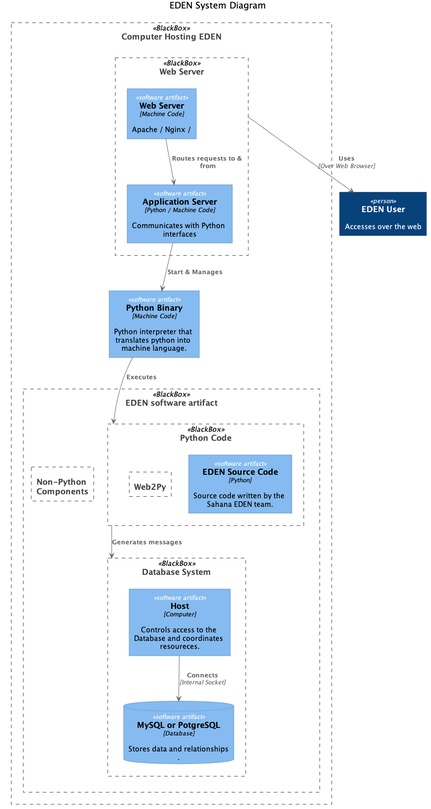
\includegraphics{images/EDEN_diagram.png}
   

   \subsection*{Why EDEN}
   I selected \acrshort{eden} for this project for two primary reasons: it is a \acrlong{foss} software project in a language I am familiar with and it is not obviously problematic. I will detail its open source pedigree shortly, but first I want to explain my second selection criteria. "Improving" software (whatever improving means) can usefully be separated into at least two questions: what quality should change and how do you bring that change about? This project attempts only to speak about the second (likely easier) question. Partially this is because the project was designed to fit within the confines of a final project for a masters degree. This project represents, roughly, three graduate level classes worth of work. I didn't feel like I had time to find \textit{and} fix flaws. So this project should be understood as neutral on the question of, "is \acrshort{eden} good?" Nothing about \acrshort{eden} seems bad to me. They have received numerous awards, glowing testimonials, and are used by many large organizations that could use other products if \acrshort{eden} were lacking. 

   I lack the experience and expertise to say that I think \acrshort{eden} is \textit{good}. Assessing if software is "good" or "bad" is not straightforward. Simply examining \glspl{sa} in isolation tell us very little. It's only through engaging with one or more \gls{sa}(s) as they exist in the lived world and contextualizing that with detailed ethnographic work that it's possible to start making value judgments \citep{Eubanks2018-hc,Schull2012-nc}. Those judgments wouldn't be universal, of course, but would be about a particular population. So this paper is done from the perspective that \acrshort{eden} seems fine to me. The project is interested in the technical details of how the \acrshort{eden} \gls{sa} emerges out of its \gls{so} and how agency is modified by that process. 

   Finally, and briefly, this project does not take the position that the technical qualities it investigates are free from the impact of social structures. \citet{Gabriella_Coleman2012-lq} and \citet{Kelty2008-jm} have both compellingly shown that the social and technical co-produce each other. However, we can still usefully speak about qualities that technical systems have and how those qualities impact our lived experience. That this project has obvious extensions in the social and ethnographic realm is a strength and declining to investigate them should be understood as a concession to time.

   \subsection*{Out of Many, One}
   Wherever possible, \acrshort{eden} uses \acrshort{foss} technologies. The language it is written in, the libraries it relies on to provide functionality, the tools it uses to support its functionality, and its main operating system are all both open source and available at no cost. \acrshort{eden} will generally operate on top of non-\acrshort{foss} systems like Microsoft Windows, but the team doesn't prioritize systems outside of the \acrshort{foss} systems they develop and test on \citep{Sahana_Foundation2015-zs}. \citet{Kelty2008-jm} talks about how \acrshort{foss} is both a philosophy and a system of development that has practical impacts. One of the side effects of \acrshort{eden} committing to use the \acrshort{foss} ecosystem is it makes my form of engagement possible. Though it is possible to examine compiled machine code and draw some conclusions about the intent and process that assembled it, such a project would be far outside my capabilities. Instead, the source code of \acrshort{eden}, web2py (the \gls{web framework} \acrshort{eden} uses), Python (the language \acrshort{eden} and web2py are written in) and all of the libraries used by the project are open source. Their preferred databases (MySql or PostgreSQL) are also fully open source projects. Open source projects often don't just publish the current source code, but offer full histories of what change, when it changed, who changed it and how it was changed. These changes often include notes about why \textit{that particular} change was made over any other possible change \citep[p. 13-16]{Chacon2014-im}. Open source projects also commonly have systems for tracking lists of unfixed flaws as well as planned future improvements (both types of \citet{Mackenzie2006-hb} relationships), but those systems operate above the layer of source code so this project does not engage with them.

  \section*{Investigating EDEN}
   My work began, as all software work does, with work of assembling the components that transform \acrshort{eden} from a collection of \gls{python} source files into a \gls{sa}. This requires connecting a number of components together: libraries and tools in the gls{python} language and a wider set of heterogeneous tools (databases, non-\gls{python} libraries and tools). Some of these components remain as source code to be interpreted by \gls{python}, some of them are downloaded as source code and go through their own assembly process to generate their own \glspl{sa}. The assembly process that draws the components of \acrshort{eden} together does not happen in a single step, but is a number of loosely ordered heterogeneous processes. Some must be completed before others and there is an officially recommended order in which to prepare the various components, but often these orders are more matters of preference than necessity. What is important is that all of the required components are collected in their expected places by the time \acrshort{eden} itself is run. 

   The \gls{sf} recommends that developers use a \gls{vm} that has \acrshort{eden} and its supporting libraries installed through a script. However, at the time that I engaged with the project, the instructions for how to install \acrshort{eden} focused on using operating systems and \gls{python} versions that have since stopped being updated\sepfootnote{softwareupdates}. Though more modern scripts can be found, the standard install scripts for the \acrshort{eden} \gls{vm} and the script to install the software on a physical machine both use operating systems released in the mid-2010s that have not been maintained for at least 5 years \citep{Canonical2020-ru}. However, \acrshort{eden} is aware that this is problematic and makes an effort to support newer versions of \gls{python} and newer operating systems, but official instructions to use the latest software are sparse.

   Choosing to offer a fixed and unusually old set of tools is the first materialized I found encoded into \acrshort{eden}\sepfootnote{whatiseden}. The state of the scripts reflect a culturally important choice. The team could note and situate their approach in their documentation, but they have not. However, project-wise choices to use older or newer versions of tools are common. There are software projects (sometimes entire programming languages) that greatly value using the most up to date version of a tool or library \citep{Fernandes_da_Costa2017-mh}. These communities have legitimate fear that older versions of tools are examined less often and will likely be fixed less frequently. They feel that using the latest (within reason) version is a goodness in of itself\sepfootnote{releaselanguage}. If the \acrshort{eden} team followed this philosophy, they would not default to using older operating systems and versions of \gls{python}. They would need to watch their ecosystem of tools and libraries more closely, but the versions they were watching would also be more in the collective consciousness of the \acrshort{foss} world. 

   All this isn't to say that the \acrshort{eden} team choice isn't a sensible one. The latest versions of tools often lose track of the world outside the top of the capitalist pyramid. The same networks of power that structure the spread of physical technology also shape the attention of active software engineers. \acrshort{eden} has chosen to use established and well-supported versions of their tools\sepfootnote{stablecaveat}. Their older set of tools is more likely to have undiscovered (or unpatched) security vulnerabilities, but they are virtually certain to function properly and immediately allow the successful assembly of an \acrshort{eden} \gls{sa}. That set of probabilities seems very well suited to the expected audience for individuals first setting up their own copies of \acrshort{eden}: individual developers setting the system up to better understand it. When another team decides to deploy their own copy of \acrshort{eden} in a way that's available to the public, they can assemble that \gls{sa} using a balance of newness and stability that feels comfortable to them\sepfootnote{updaterisk}. 

   \subsection*{Investigating Assembly}
   It's one thing to identify where the \acrshort{eden} install scripts sit in a cultural gradient. It's another to engage the particular choices that the \acrshort{eden} project has made. I chose to install a far newer set of tools, based on the projects newest recommendations for new installs \citep{Konig2019-ya}. I was guided by the \gls{python} 2.7 installation script provided on the Sahana \acrshort{eden} wiki\sepfootnote{edensetup}. However, I chose to use a version of \gls{python} originally released in 2016 (six years after the default version used by \acrshort{eden}). Using a newer version of python seemed like a sensible software engineering choice and also a way to check if \acrshort{eden} was, as they claim, able to operate equally well on the version I selected (3.6.9) and the 2.7 version that \acrshort{eden} uses by default\sepfootnote{pythonversion}.

   Selecting a more modern \gls{python} turned out to have knock-on effects. Some of the libraries that \acrshort{eden} requires are written only for \gls{python} 2.7 and replacements were needed to function with 3.6. One of the major changes was that the version of \gls{w2p} the \acrshort{eden} scripts installs does not support \gls{python} 3.6 and so I needed to chose an updated version. I selected 2.18.5, but this new combination of the \acrshort{eden} source code and the \gls{w2p} source code revealed that the two projects had drifted apart in small but essential ways. Specifically, in a section of the \gls{w2p} and \acrshort{eden} code that handled data validation.

   Data validation is, in general, the work of verifying that information conforms to a set of standards and informing the user how it has failed to conform when a problem is found. This should always be performed any time data is stored in a system. Digital storage systems have expectations that, when violated, can cause immediate systems failures. Web frameworks commonly provide facilities for verifying data and \gls{w2p} is no exception. \gls{w2p} has components that will check that that user input can be converted to numbers or dates or email addresses, among others. \gls{w2p} is open source and so all of that functionality can be expanded by programs that make use of \gls{w2p} and \acrshort{eden} does so in a number of places. 

   In between the version of \gls{w2p} that \acrshort{eden} uses by default and the version of \gls{w2p} that I selected, the control flow of data validation has changed slightly. This change meant that custom data validation classes that were written using the older \gls{w2p} system no longer fit into the expected control flow of data validation. The \acrshort{eden} data validation code, based on the older standard, is not called properly when using the newer version of \gls{w2p}. This doesn't stop the successful assembly of an \acrshort{eden} \gls{sa}, but once that \gls{sa} is assembled most of its functionality in inaccessible because the \acrshort{eden}-specific data validation code won't run and so the system won't accept that data. 

   This problem is interesting because it turns out it captures a moment in time between the \gls{w2p} team and the teams that use \gls{w2p} (i.e. \acrshort{eden}). If I had selected a slightly earlier version of \gls{w2p}, then it would have used the old system and the \acrshort{eden} code would remain functional. \gls{w2p} immediately realized the problem and accepted a fix\sepfootnote{problemfix} for the issue. This is exactly what \citet{Mackenzie2006-hb} describes when talking about the management of relationships between software components. The \gls{w2p} successfully implemented a new way of handling data validation control flow, but they neglected that they were doing it in such a way as to break an existing relationship they did not mean to break. Because I happened to select a version of \gls{w2p} that was temporarily out of relation with \acrshort{eden}, I failed to assemble a fully functional \gls{sa}. This got me interested in assembly.


   \subsection*{Investigating Assembly}


   

   
  
   \printnoidxglossaries
   \setlength{\parindent}{4em}
   \bibliography{Final_Draft}

\end{document}